\section{Degenerate Electron Gas}
The office hours for this course will be Monday 4-5pm with Marcel, and 4-5pm on Tuesday with Oguzhan.

\subsection{Introducing the Degenerate Electron Gas}
\begin{figure}[htbp]
    \centering
    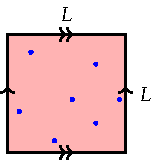
\includegraphics[]{Images/fig-jelliumcartoon.pdf}
    
    \caption{A cartoon depiction of the degenerate electron gas model. We consider a fixed, finite number of electrons $N$ in a three-dimensional box with side length $L$ and periodic boundary conditions. The electrons feel a uniformly distributed background of positive charge.}
    \label{fig-jelliumcartoon}
\end{figure}
Also known as the ``Jellium Model'', we consider a gas of electrons moving in a uniformly distributed background of positive charge. We begin with a 3d box of size $L$, and then take the thermodynamic limit of $L \to \infty$. 

We will use periodic boundary conditions, so if an electron leaves the box from one side, it comes in from the other. This is convenient as then the model admits plane waves solutions. We could use hard boundaries, and the description should agree in the $L \to \infty$ limit, but this set of boundary conditions is harder to work with; we would have cosine and and sines instead of plane waves.

The plane-wave basis will be a natural choice given the periodic BCs. Explicitly, we can write this as:
\begin{equation}
    \psi_{k, \lambda}(\v{x}) = \frac{1}{\sqrt{V}}e^{i\v{k} \cdot \v{x}}\eta_\lambda
\end{equation}
with $\lambda = (\uparrow, \downarrow)$ is the spin index. We have the spinors:
\begin{equation}
    \eta_\uparrow = \m{1\\0}, \quad \eta_\downarrow = \m{0\\1}
\end{equation}
The momentum is given by:
\begin{equation}
    \v{k} = (k_x, k_y, k_z), k_i = \frac{2\pi}{L}n_i
\end{equation}
where $n_i \in \ZZ$. The Hamiltonian is given by:
\begin{equation}
    \begin{split}
        H &= H_{el} + H_b + H_{el-b}
        \\ H_{el} &= \sum_{i=1}^N \frac{p_i^2}{2m} + \frac{1}{2}e^2\sum_{i \neq j} \frac{e^{-\mu\abs{\v{r}_i - \v{r}_j}}}{\abs{\v{r}_i - \v{r}_j}}
        \\ H_b &= \frac{1}{2}e^2 \int d^3x d^3x' \frac{n(\v{x})n(\v{x}')e^{-\mu\abs{\v{x} - \v{x}'}}}{\abs{\v{x} - \v{x}'}}
        \\ H_{el-b} &= -e\sum_{i=1}^N \int d^3x \frac{n(\v{x})e^{-\mu\abs{\v{x} - \v{r}_i}}}{\abs{\v{x} - \v{r}_i}}.
    \end{split}
\end{equation}
$H_{el}$ is just the kinetic energy of the electrons and the point-charge on point-charge interactions. $H_b$ is the electrostatic interaction of the background field with itself. And $H_{el-b}$ is the electrostatic interactions of the electrons with the background field. $N$ is the number of electrons, $V = L^3$ is the volume, $n = N/V$ is the electron density, and $\mu$ is a convergence factor which we send $\mu \to 0$\footnote{In nuclear physics this has significance as the \emph{Yukawa potential}; here we just use it as a convenient trick to remove some diverging integrals}. 

\subsection{Simplifying the background terms}
We want to rewrite this in second quantization notation. Only $H_e$ will have nontrivial structure in the second quantization notation, but nevertheless the other terms are necessary for the stability of the system.

Let us start with the second term, which is the simplest. We deal with a uniform background density, namely $n(\v{x}) = n = N/V$. $H_b$ then becomes a simple integral:
\begin{equation}
    \begin{split}
        H_b &= \frac{1}{2}e^2\left(\frac{N}{V}\right)^2 \int d^3x \int d^3 x' \frac{e^{-\mu\abs{\v{x} - \v{x}'}}}{\abs{\v{x} - \v{x}'}}.
        \\ &= \frac{1}{2}e^2\left(\frac{N}{V}\right)^2 \int d^3x \int d^3z \frac{e^{-\mu z}}{z}
        \\ &= \frac{1}{2}e^{2}\left(\frac{N^2}{V}\right)\frac{4\pi}{\mu^2}
    \end{split}
\end{equation}
Where in the second equality we use $z = \v{x}' - \v{x}$ in order to make the integrals independent, and evaluate the integrals in the third equality (the inner integral evaluating to $\frac{4\pi}{\mu^2}$, the outer to $V$). We can see why it was useful to introduce the $e^{-\mu}$; the integral would have diverged otherwise due to the long-range nature of the Coloumb interaction. Note also that we performed the integral assuming $\mu^{-1} \ll L$. We can similarly calculate $H_{el-b}$:
\begin{equation}
    \begin{split}
        H_{el-b} &= -e\frac{N}{V}\sum_{i=1}^N \int d^3x \frac{e^{-\mu\abs{\v{x} - \v{r}_i}}}{\abs{\v{x} - \v{r}_i}}
        \\ &= -e\frac{N}{V}\sum_{i=1}^N \int d^3z \frac{e^{-\mu z}}{z}
        \\ &= -e^2 \frac{N}{V} N \int d^3z\frac{e^{-\mu z}}{z}
        \\ &= -e^2\frac{N^2}{V}\frac{4\pi}{\mu^2}
    \end{split}
\end{equation}
We note the partial cancellation of the $H_b$ and the $H_{el-b}$ terms of the Hamiltonian; we will see another cancellation later.

A reasonable question is why the $\mu^{-1} \ll L$ assumption is necessary. It boils down to the the fact that we have periodic boundary conductions, and we do \emph{not} want the electric field of a given electron to interact with itself (or at least, not in a way that is exponentially insignificant and hence ignorable). See Fig. \ref{fig-jelliumlengthassumption} below for a visual demonstration of the importance of this assumption.

\begin{figure}[htbp]
    \centering
    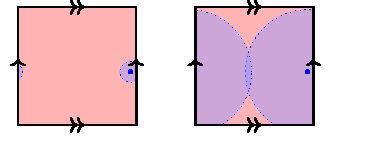
\includegraphics[]{Images/fig-jelliumlengthassumption.pdf}
    
    \caption{Comparisons of ``spheres of interaction'' of electrons when $\mu^{-1} \ll L$ (left) and $\mu^{-1} \sim L$ (right). We can see that in the former case, the electron does not interact with itself through the periodic boundary condition (beyond a negligeble exponentially small contribution), and so the system is physically sound. In the latter case, the electron does have a nontrivial interaction with its own electric field, as seen through the overlap of the sphere of interaction; this is not physical. Hence in our analysis of the Jellium model, we make the assumption that $\mu^{-1} \ll L$.}
    \label{fig-jelliumlengthassumption}
\end{figure}

With these simplifications, 
\begin{equation}
    H = -\frac{1}{2}e^2\frac{N^2}{V}\frac{4\pi}{\mu^2} + H_{el}
\end{equation}
Note that all of the interesting physics is contained in $H_{el}$, but we need $H_b + H_{el}$ to get a finite theory; we can see that if we took $\mu \to 0$ now, the energy would diverge; presumably there will be some sort of cancellation that occurs with $H_{el}$ that will regularize the theory. 

\subsection{Second Quantization of the Electron Term}
Let us now transform the $H_{el}$ term into second quantized notation.
\begin{enumerate}[(i)]
    \item We start with the kinetic energy term:
    \begin{equation}
        \begin{split}
            \bra{\v{k}_1\lambda_1}T\ket{\v{k}_2\lambda_2} &= \frac{1}{2mV}\int d^3x e^{-i\v{k} \cdot \v{x}}\eta_{\lambda_1}^\dag (-\hbar^2\nabla^2)e^{i\v{k}_2\cdot \v{x}}\eta_{\lambda_2}
            \\ &= \frac{\hbar^2 k_2^2}{2mV}\delta_{\lambda_1\lambda_2}\int d^3x e^{-i\v{x} \cdot (\v{k}_1 - \v{k_2})}
            \\ &= \frac{\hbar^2k_2^2}{2m}\delta_{\lambda_1\lambda_2}\delta_{\v{k}_1\v{k}_2}
        \end{split}
    \end{equation}
    where we use that $\int d^3x e^{-i\v{x} \cdot (\v{k}_1 - \v{k_2})} = V\delta_{k_1k_2}$. Wee therefore obtain:
    \begin{equation}
        \hat{T} = \sum_{k, \lambda}\frac{\hbar^2 k^2}{2m}c_{k\lambda}^\dag c_{k\lambda}.
    \end{equation}
    \item We now look at the potential term:
    \begin{equation}
        \bra{k_1\lambda_1k_2\lambda_2}V\ket{k_3\lambda_3k_4\lambda_4} = \frac{e^2}{V}\delta_{\lambda_1\lambda_3}\delta_{\lambda_2\lambda_4}\delta_{k_1 + k_2, k_3 + k_4}\frac{4\pi}{(\v{k}_1 - \v{k}_3)^2 + \mu}.
    \end{equation}
    See F\&W for details; there is nothing conceptually new in the calculation above, it is only slightly more annoying at there are four plane wave terms.
\end{enumerate}
We therefore obtain:
\begin{equation}\label{eq-JelliumquantizedH}
    \hat{H} = \hat{T} - \frac{1}{2}\frac{e^2N^2}{V}\frac{4\pi}{\mu} + \frac{e^2}{2V}\sum_{k, \lambda}\delta_{\lambda_1\lambda_3}\delta_{\lambda_2\lambda_4}\delta_{k_1 + k_2, k_3 + k_4}\frac{4\pi}{(\v{k}_1 - \v{k}_3)^2 + \mu} c^\dag_{k_1\lambda_1}c^\dag_{k_2\lambda_2}c_{k_4\lambda_4}c_{k_3\lambda_3}.
\end{equation}
Now we have to think a little bit; we have three delta functions, two for spin, one for momenta. We can explicitly two summations over $\lambda$ and one over momentum. Instead of doing so blindly, we will find it useful to make the following change of variables:
\begin{equation}
    \m{\v{k}_1 = \v{k} + \v{q} & \v{k}_3 = \v{k} \\ \v{k}_2 = \v{p} - \v{q} & \v{k}_4 = \v{p}} \quad \m{\lambda_1 = \alpha \\ \lambda_2 = \beta}
\end{equation}
We may notice that we express the four momenta in terms of three, but this is ok; we have the extra constraint on the momentum already, and it was designed to satisfy this constraint. Substituting, the potential term becomes:
\begin{equation}
    \frac{e^2}{2V}\sum_{\v{k}\v{p}\v{q}}\sum_{\alpha\beta}\frac{4\pi}{\v{q}^2 + \mu^2}c^\dag_{\v{k} + \v{q}\alpha}c^{\dag}_{\v{p} - \v{q}\beta}c_{\v{p}\beta}c_{\v{k}\alpha}.
\end{equation}
We now want to send $\mu \to 0$. Note that we can do this for any term in the sum for which $\v{q} \neq \v{0}$. The only singular term is $\v{q} = \v{0}$, so let us study that term:
\begin{equation}\label{eq-badtermJellium}
    \begin{split}
        \frac{e^2}{2V}\sum_{\v{k}\v{p}}\sum_{\alpha\beta}\frac{4\pi}{\mu^2}c^\dag_{\v{k}\alpha}c^{\dag}_{\v{p}\beta}c_{\v{p}\beta}c_{\v{k}\alpha} &= \frac{e^2}{2V}\sum_{\v{k}\v{p}}\sum_{\alpha\beta}\frac{4\pi}{\mu^2}c^\dag_{\v{k}\alpha}(c_{\v{k}\alpha}c^\dag_{\v{p}\beta} - \delta_{\v{k}\v{p}}\delta_{\alpha\beta})c_{\v{p}\beta}
        \\ &= \frac{e^2}{2V}\frac{4\pi}{\mu^2}(\hat{N}^2 - \hat{N})
        \\ &=\frac{e^2}{2}\frac{N^2}{V}\frac{4\pi}{\mu^2} - \frac{e^2}{2}\frac{N}{V}\frac{4\pi}{\mu^2}
    \end{split}
\end{equation}
where in the first equality we have commuted the $c_{\v{k}\alpha}$ between the two $c^\dag$s (being careful to respect the commutation relations), in the second equality we have used the definition of the number operator, and in the third equality we used the fact that we work with a system with a finite, fixed number of electrons and hence we can replace the operators $\hat{N}$ with the number of particles $N$. 

We see that the first term in Eq. \eqref{eq-badtermJellium} and the second term in Eq. \eqref{eq-JelliumquantizedH} cancel. We argue that the second term in Eq. \eqref{eq-badtermJellium} is vanishingly small in the thermodynamic limit. We argue this as follows; since $N/V$ (the number density) is constant with the system size, the term is constant with the system size; however $\avg{H}$ is extensive, and scales with the system size ($\avg{H} \sim V \sim N$). Hence we may choose to ignore it. So let us conclude by stating our final Hamiltonian:
\begin{equation}
    \hat{H} = \sum_{\v{k}\alpha}\frac{\hbar^2\v{k}^2}{2m}c^\dag_{\v{k}\lambda}c_{\v{k}\lambda} + \frac{e^2}{2V}\sum_{\v{k}\v{p}\v{q}}'\sum_{\alpha\beta} \frac{4\pi}{\v{q}^2}c^\dag_{\v{k} + \v{q}\alpha}c^{\dag}_{\v{p} - \v{q}\beta}c_{\v{p}\beta}c_{\v{k}\alpha}
\end{equation}
where the prime on the summation denotes that we do not include the $\v{q} = 0$ term.

\subsection{Rescaling the Hamiltonian}
It is possible to gain important insights by introducing ``natural'' dimensionless variables. We define the inter-electron spacing $r_0$ as the radius of the sphere corresponding to the volume per electron. We then define the dimensionless quantity $r_s$ as the ratio of $r_0$ with the Bohr radius $a_0$:
\begin{equation}
    \begin{split}
        &\frac{V}{N} = \frac{4}{3}\pi r_0^3
        \\ &a_0 = \frac{\hbar^2}{me^2}
        \\ &\boxed{r_s = \frac{r_0}{a_0} \approx 2-6 \text{ for metals}}
    \end{split}
\end{equation}
The above are very good things to remember; there will be questions about them on the midterm and final!
Based on these, let us define:
\begin{equation}
    \bar{V} = V/r_0^3, \bar{\v{k}} = \v{k}r_0
\end{equation}
So our rescaled Hamiltonian can be written as:
\begin{equation}
    \hat{H} = \frac{e^2}{a_0r_s^2}\left(\sum_{\bar{\v{k}}\alpha} \frac{\bar{\v{k}}^2}{2}c^\dag_{\bar{\v{k}}\lambda}c_{\bar{\v{k}}\lambda} + \frac{e^2}{2\bar{V}}\sum_{\bar{\v{k}}\bar{\v{p}}\bar{\v{q}}}'\sum_{\alpha\beta} \frac{4\pi}{\bar{\v{q}}^2}c^\dag_{\bar{\v{k}} + \bar{\v{q}}\alpha}c^{\dag}_{\bar{\v{p}} - \bar{\v{q}}\beta}c_{\bar{\v{p}}\beta}c_{\bar{\v{k}}\alpha}\right)
\end{equation}
where $\frac{e^2}{a_0} \approx 13.6\si{eV}$ is the Rydberg constant/hydrogen binding energy. This result shows that \underline{in the $r_s \to 0$} \underline{(high density) limit, the electron-electron interaction becomes weak.} This is very counterintutive; in classical physics, the electron-electron interaction would dominate! Another thing to note; starting from the high-density limit, we can solve an easy problem (one that just contains the kinetic energy of the electrons) and then treat the electron-electron interactions as a small perturbation (can be reasonably treated in perturbation theory, expanding in powers of $r_s$). The actual series for the ground-state energy reads:
\begin{equation}
    E_G = \frac{Ne^2}{a_0r_s^2}\left(a + br_s + cr_s^2 \log(r_s) + dr_s^2 + \cdots\right)
\end{equation}
the $\log(r_s)$ term is perhaps a bit peculiar, but indeed if we do the perturbation expansion diligently we can confirm that it shows up. In the following, we will find $a$ and $b$. We also remark that $c$ may be similarly obtained, but $d$ and higher powers require more advanced techniques, namely Green's function techniques\footnote{Green's functions give us a way to do a more formalized version of perturbation theory. With them, the expansion has been computed to seventh order; but the computation becomes much more difficult as we add higher order terms.}. We now proceed with the perturbation theory.

\subsection{Perturbation Theory (High Density)}
We return to our non-rescaled Hamiltonian so as to avoid having to write bars all the time. We split the Hamiltonian into two parts (the kinetic energy term and the perturbing electron-electron term):
\begin{equation}
    \begin{split}
        \hat{H}_0 &= \sum_{\v{k}\alpha}\frac{\hbar^2\v{k}^2}{2m}c^\dag_{\v{k}\lambda}c_{\v{k}\lambda}
        \\ \hat{H_1} &= \frac{e^2}{2V}\sum_{\v{k}\v{p}\v{q}}'\sum_{\alpha\beta} \frac{4\pi}{\v{q}^2}c^\dag_{\v{k} + \v{q}\alpha}c^{\dag}_{\v{p} - \v{q}\beta}c_{\v{p}\beta}c_{\v{k}\alpha}
    \end{split}
\end{equation} 

\subsubsection{Zeroth Order}
The ground state of $\hat{H_0}$ can be written as:
\begin{equation}
    \ket{F} = \prod_{\abs{\v{k}} < k_F} c^\dag_{\v{k} \uparrow}c^{\dag}_{\v{k}\downarrow}\ket{0}.
\end{equation}
For $N$ electrons, the Fermi momentum is determined by:
\begin{equation}
    N = \bra{F}\hat{N}\ket{F} = \sum_{\v{k}\lambda}\bra{F}n_{\v{k}\lambda}\ket{F} = \sum_{\v{k}\lambda}\theta(k_F - \abs{\v{k}}) = 2V\int \frac{d^3k}{(2\pi)^{3}}\theta(k_F - \abs{\v{k}}) = \frac{2V}{(2\pi)^3}\left(\frac{4}{3}\pi k_F^3\right) = \frac{V}{3\pi^2}k_F^3
\end{equation}
We have therefore obtained $k_F$ defined by electron density. In the above we have used the standard perscription:
\begin{equation}
    \frac{1}{V}\sum_{\v{k}} \to \int \frac{d^3k}{(2\pi)^3}
\end{equation}
and the step function:
\begin{align*}
    \theta(x) = \begin{cases}
        1 & x > 0
        \\ 0 & x < 0.
    \end{cases}
\end{align*}
We can now solve for $k_F$:
\begin{equation}
    k_F = \left(\frac{3\pi^2 N}{V}\right)^{1/3} = \left(\frac{9\pi}{4}\right)^{1/3}r_0^{-1} \approx 1.92 r_0^{-1}
\end{equation}
which tells us that $k_F$ is (up to a factor of order unity) equal to the inverse of $r_0$. One can use the above to relate conduction bands and $k_F$ to the lattice spacing, among other useful applications. So now doing the ground state energy calculation, we have:

\begin{equation}
    \begin{split}
        E^{(0)} = \bra{F}\hat{H}_0\ket{F} = \frac{\hbar^2}{2m}\sum_{\v{k}, \alpha}\bra{F}n_{\v{k}\alpha}\ket{F}\v{k}^2 = \frac{\hbar^2}{2m}\sum_{\v{k}, \alpha}\v{k}^2\theta(k_F - \abs{\v{k}}) &= \frac{\hbar^2}{2m}2\frac{V}{(2\pi)^3}\int d^3k \v{k}^2\theta(k_F - \v{k})
        \\ &= \frac{3}{5}\frac{\hbar^2k_F^2}{2m}N
        \\ &= \frac{3}{5}\e_F N
        \\ &= \left(\frac{e^2}{2a_0}\right)N\frac{2.21}{r_s^2}
    \end{split}
\end{equation}
where in the fourth equality the factor of 2 comes from the summation over spin, and the integral is performed by going into spherical coordinates. Again $\frac{e^2}{2a_0} = 13.6\si{eV}$ is the Rydberg constant. This tells us that for metals (i.e. $r_s \approx 2-6$), the energy of electrons is on the order of $\si{eV}$.

\subsubsection{First Order}
To first order, we simply calculate the expectation value:
\begin{equation}
    E^{(1)} = \bra{F}\hat{H}_1\ket{F} = \frac{e^2}{2V}\sum_{\v{k}\v{p}\v{q}}'\sum_{\alpha\beta}\bra{F}c^\dag_{\v{k} + \v{q}\alpha}c^{\dag}_{\v{p} - \v{q}\beta}c_{\v{p}\beta}c_{\v{k}\alpha}\ket{F}.
\end{equation}
The above is more complicated; we must deal with the four-fermion operator acting on the ground state. We can do this the hard way; we can substitute in the ground state and use commutation relations amongst the operators. Or, we can give a slick argument that does the same job but with less writing; let's do it this way. We start with a Fermi sphere filled with electrons. The annhilation operators can only remove two electrons from inside the spheres, and the creation operators can either create electrons where they are removed, or create them elsewhere. If they are created elsewhere, the state we end up with will be orthogonal to the ground state $\ket{F}$. So, the only nonvanishing constributions will come from the terms where the annhilation operators remove electrons from inside the sphere, and the creation operators fill back in the holes (giving us back $\ket{F}$, up to some prefactor).

\begin{figure}[htbp]
    \centering
    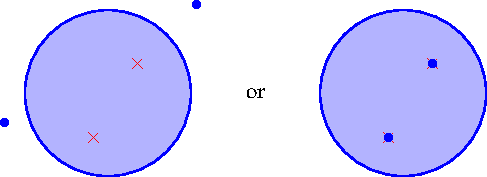
\includegraphics[]{Images/fig-fourfermionopargument.pdf}
    \caption{Action of the 4 fermion operators on the ground state $\ket{F}$. The two annihilation operators remove some pair of fermions within the Fermi sphere. The creation operators can then create fermions elsewhere (left), in which case the final state is orthogonal to $\ket{F}$ and does not contribute to the expectation value. Alternatively, the creation operators can fill the holes created by the annhilation operators (right), in which case the final state is proportional to $\ket{F}$ and hence does contribute to the expectation value.}
    \label{fig-fourfermionopargument}
\end{figure}

There are two pairings of the creation/annhilation operators for which the above can occur.  The first possibility is:
\begin{equation}
    \m{\v{k} + \v{q}, \alpha = \v{k}, \alpha
    \\ \v{p} - \v{q}, \beta = \v{p}, \beta} \quad \text{or} \quad \m{\v{k} + \v{q}, \alpha = \v{p}, \beta
    \\ \v{p} - \v{q}, \beta = \v{k}, \alpha}
\end{equation}
If we look at the first possibility, we immediately obtain the constraint that $\v{q} = 0$. However, we have already removed all such terms in our sum (note the prime); so the only the second possibility contributes. We call this the ``exchange term'', because the spins are exchanged. The conclusion of this argument is that the terms of the sum are only nonzero when the exchange conditions of $\v{k} + \v{q} = \v{p}, \alpha = \beta$ are satisfied. We can now use this to compute the first order correction to the GS energy:
\begin{equation}
    \begin{split}
        E^{(1)} &= \frac{e^2}{2V}\sum_{\v{k}\v{p}\v{q}}'\sum_{\alpha\beta} \delta_{\v{k} + \v{q}, \v{p}}\delta_{\alpha\beta} \bra{F}c^\dag_{\v{k} + \v{q}\alpha}c^{\dag}_{\v{p} - \v{q}\beta}c_{\v{p}\beta}c_{\v{k}\alpha}\ket{F}\frac{4\pi}{\v{q}^2}
        \\ &= \frac{e^2}{2V}\sum_{\v{k}\v{p}\v{q}}'\sum_{\alpha\beta} \delta_{\v{k} + \v{q}, \v{p}}\delta_{\alpha\beta} \bra{F}c^\dag_{\v{k} + \v{q}\alpha}c^{\dag}_{\v{k}\alpha}c_{\v{k} + \v{q}\alpha}c_{\v{k}\alpha}\ket{F}\frac{4\pi}{\v{q}^2}
        \\ &= -\frac{e^2}{2V}\sum'_{\v{k}\v{q}}
        \sum_\alpha\bra{F}\hat{n}_{\v{k} + \v{q} \alpha}\hat{n}_{\v{k}\alpha}\ket{F}\frac{4\pi}{\v{q}^2}
        \\ &= -\frac{e^2}{2V}\sum_{\v{k}\v{q}}'\sum_\alpha \frac{4\pi}{\v{q}^2}\theta(k_F - \abs{\v{k} + \v{q}})\theta(k_F - k)
        \\ &= -\frac{e^2}{2}\frac{4\pi V}{(2\pi)^6}\int d^3k \int d^3q\frac{1}{\v{q}^2} \theta(k_F - \abs{\v{k} + \v{q}})\theta(k_F - k)
    \end{split}
\end{equation}
We make a change of variables $\v{k} \to \v{p} = \v{k} + \frac{1}{2}\v{q}$. This yields:
\begin{equation}
    \begin{split}
        E^{(1)} &= -\frac{4\pi e^2V}{(2\pi)^6}\int d^3 q \frac{1}{\v{q}^2}\int d^3p \theta(k_F - \abs{\v{p} + \frac{1}{2}\v{q}})\theta(k_F - \abs{\v{p} - \frac{1}{2}\v{q}})
    \end{split}
\end{equation}
This integral is much more symmetric; if we think about this geometrically, we are looking at the overlap of spheres when we calculate the inner integral over $q$:

\begin{figure}[htbp]
    \centering
    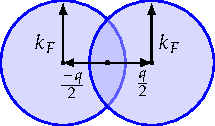
\includegraphics[]{Images/fig-twosphereoverlap.pdf}

    \caption{Visualization of the integral $I(q) = \int d^3p \theta(k_F - \abs{\v{p} + \frac{1}{2}\v{q}})\theta(k_F - \abs{\v{p} - \frac{1}{2}\v{q}})$. The two step functions correspond to the two spheres shown above, and the overall integral calculates their overlap in volume.}
    \label{fig-twosphereoverlap}
\end{figure}

The integral is a standard exercise in multivariable calculus. One finds:
\begin{equation}
    \int d^3p \theta(k_F - \abs{\v{p} + \frac{1}{2}\v{q}})\theta(k_F - \abs{\v{p} - \frac{1}{2}\v{q}}) = \frac{4\pi}{3}k_F^3\left(1 - \frac{3}{2}x + \frac{1}{2}x^2\right)\theta(1 - x), \quad x = \frac{q}{2k_F}.
\end{equation}
where the $\theta$ function is there to account for the fact that when $q$ is sufficiently large the spheres do not touch. We now calculate the outer integral. We make the observation that in spherical coordinates, $d^3q \to 4\pi q^2 dq$ and so the $q^2$ in the denominator cancels. All we have to do is just an integral of a polynomial; child's play. We are left with:
\begin{equation}
    E^{(1)} = -\frac{e^2}{2a_0}\frac{N}{r_s}\left(\frac{9\pi}{4}\right)^{1/2}\frac{3}{2\pi} = -\frac{e^2}{2a_0}N\frac{0.916}{r_s}.
\end{equation}

\subsubsection{Combining Results}
In summary, the total ground state energy (to first order) is:
\begin{equation}\label{eq-pertresultjellium}
    \frac{E}{N} = \frac{e^2}{2a_0}\frac{1}{r_s^2}\left(2.21 - 0.916r_S + \ldots\right)
\end{equation}
We identify the first term as the free Fermi gas energy, and the second term as the exchange energy.

A comment: We have done perturbation theory in $r_s$ which we have treated as ``small'', but really $r_s$ is $2-6$ for metals so it is not really small. It surprisingly works fairly well, anyway.

\subsection{The Variational Viewpoint}
We now switch perspectives a little bit, and find that we can learn something more interesting about the calculation we just did. We viewed it as a perturbation theory expansion in $r_s$. But we can view it instead as a variational calculation.

Recall the variational principle:
\begin{align*}
    E_{GS} \leq \bra{\psi}H\ket{\psi}
\end{align*}
where $H$ is a Hamiltonian, $\ket{\psi}$ is any state, and $E_{GS}$ is the ground state energy of $H$. In our case, we have calculated $\bra{F}\hat{H}_0 + \hat{H}_1\ket{F}$, which can also be viewed as a variational energy parametrized by electron density $r_s$. Taking our result from Eq. \eqref{eq-pertresultjellium}, we can plot an energy landscape as a function of $r_s$:

\begin{figure}[htbp]
    \centering
    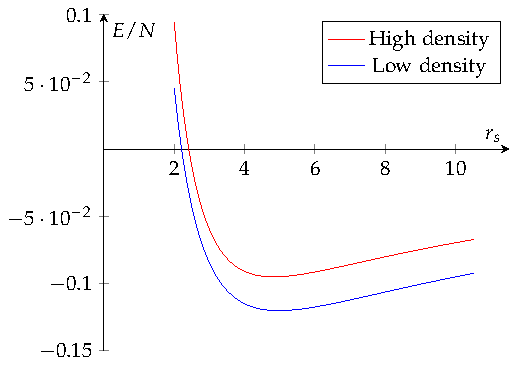
\includegraphics[]{Images/fig-jelliumenergylandscape.pdf}

    \caption{Plot of the variational energy landscape for. $E/N$ is in units of $e^2/2a_0$, and we plot in a range of typical $r_s$ for metals. In red we plot the first-order perturbation expansion for $E/N$ in the high-density limit (Eq. \eqref{eq-pertresultjellium}). In blue we plot the first-order perturbation expansion for $E/N$ in the low-density limit (Eq. \eqref{eq-pertresultjelliumlowdensity}). We can find the $r_s$ that minimizes $E/N$ to approximate the true ground state energy (i.e. the binding energy per electron in metals).}
    \label{fig-jelliumenergylandscape}
\end{figure}

We find that the $r_s$ that minimizes this energy is $(r_s)_{\min} = 4.83$ and $E_{\min}/N = -0.095\frac{e^2}{2a_0} \approx -1.29\si{eV}$. For comparison, the binding energy per electron in sodium (found experimentally) is $r_s = 3.86$ and $E/N = -1.13\si{eV}$. Even this very simple calculation gets us the correct order of magnitude.

\subsection{Perturbation Theory (Low Density)}
It turns out that we can do perturbation theory also in the large $r_s$/low-density limit, where we take:
\begin{align*}
    \hat{H}_0 &= \frac{e^2}{2V}\sum_{\v{k}\v{p}\v{q}}'\sum_{\alpha\beta} \frac{4\pi}{\v{q}^2}c^\dag_{\v{k} + \v{q}\alpha}c^{\dag}_{\v{p} - \v{q}\beta}c_{\v{p}\beta}c_{\v{k}\alpha}
    \\ \hat{H_1} &= \sum_{\v{k}\alpha}\frac{\hbar^2\v{k}^2}{2m}c^\dag_{\v{k}\lambda}c_{\v{k}\lambda}
\end{align*}
i.e. we exchange which is the dominant and which is the perturbing Hamiltonian. In this limit, we find (though the calculation is more difficult):
\begin{equation}\label{eq-pertresultjelliumlowdensity}
    \frac{E}{N} = \frac{e^2}{2a_0}\frac{1}{r_s}\left(-1.79 + \frac{2.66}{\sqrt{r_s}} + \ldots \right)
\end{equation}
This is plotted as the dashed line in the figure above. This is the controversial ``Wigner crystal''; it is not known if this actually applied, as the crystallization of electrons has never been observed in three dimensions.

Next class, we will look at the Hartree-Fock approximation.